\documentclass{article}
\usepackage[%
    left=0.5in,%
    right=0.5in,%
    top=0.5in,%
    bottom=0.5in,%
]{geometry}%
\usepackage{minitoc}
\usepackage{multicol}
\usepackage{graphicx}
\usepackage{fixltx2e}
\usepackage{hyperref}
\usepackage{hyperref}
    \hypersetup{ colorlinks = true, linkcolor = blue }
\usepackage{blindtext}

\graphicspath{ {./} }

\newcommand{\inlinecode}[2]{\colorbox{lightgray}{\lstinline
[language=#1]$#2$}}
\newcommand{\worddef}[1]{\hyperref[sec:reference]{\textit{#1}}}

\begin{document}

\section{Relocation and Protection}
\subsection{Principles}
\begin{flushleft}
\textbf{Relocation}: when a program is run, it \textbf{does not know} in advance which partition/addresses it will occupy.
\begin{itemize}
	\item The program \textbf{cannot} simply generate static addresses (e.g. jump instructions) that are absolute
	\item Addresses should be \textbf{relative} to where the program has been loaded.
	\item Relocation must be solved in an operating system that allows processes to run at \textbf{changing memory} locations
\end{itemize}
\textbf{Protection}: once you can have two programs in memory at the same time, protection must be enforced
\end{flushleft}

\subsection{Address types}
\begin{flushleft}
A \textit{logical address} is a memory address seen by the process.
\begin{itemize}
	\item It is \textbf{independent} of the current physical memory assignment
	\item It is, e.g., \textbf{relative} to the start of the program 
\end{itemize}
A \textit{physical address} refers to an \textbf{actual location} in main memory.
\begin{itemize}
	\item The logical address space must be \textbf{mapped onto} the machine’s physical address space
\end{itemize}
\end{flushleft}

\subsection{Approaches}
\begin{itemize}
	\item \textit{Static “relocation”} at \textbf{compile} time: a process has to be located at the same location every single time (impractical)
	\item \textit{Dynamic relocation} at \textbf{load} time. An \textbf{offset} is added to every logical address to account for its physical location in memory. Slows down the loading of a process, \textbf{does not account} for swapping
	\item \textit{Dynamic relocation} at \textbf{runtime}
\end{itemize}

\subsection{At Runtime: Base and Limit Registers}
\begin{flushleft}
\begin{itemize}
	\item Two special purpose registers are maintained in the \textbf{CPU} (the \textbf{MMU}), containing a \textbf{base address} and \textbf{limit}
	\item The base register stores the \textbf{start address} of the partition. The limit register holds the \textbf{size} of the partition 
	\item \textbf{At runtime}: The base register is \textbf{added to the logical} (relative) address to generate the physical address. The resulting address is compared against the limit register.
\end{itemize}
This approach \textbf{requires} hardware support (was not always present in the early days!)
\end{flushleft}

\section{Dynamic partinioning}
\subsection{Context}
\begin{flushleft}
\textbf{Fixed partitioning} results in \textit{internal fragmentation}:
\begin{itemize}
	\item An exact match between the requirements of the process and the available partitions may not exist
	\item The partition may not be used entirely 
\end{itemize}
\textbf{Dynamic partitioning}:
\begin{itemize}
	\item A variable number of partitions of which the size and starting address can \textbf{change} over time
	\item A process is allocated the \textbf{exact amount} of \textbf{contiguous} memory it requires, thereby preventing internal fragmentation.
\end{itemize}
\end{flushleft}

\subsection{Swapping}
\begin{flushleft}
\textit{Swapping} holds some of the processes \textbf{on the drive} and \textbf{shuttles} processes between the drive and main memory as necessary.\\
\textbf{Reasons} for swapping:
\begin{itemize}
	\item Some processes only run occasionally
	\item We have more processes than partitions (assuming fixed partitions)
	\item A process’s memory requirements have changed, e.g. increased
	\item The total amount of memory that is required for the processes exceeds the available memory
\end{itemize}
\end{flushleft}

\subsection{Difficulties}
\begin{flushleft}
\textbf{External fragmentation}:
\begin{itemize}
	\item Swapping a process out of memory will create \textbf{“a hole”}
	\item A new process may not use the entire “hole”, leaving a small unused block
	\item A new process may be too large for a given a “hole”
\end{itemize}
\textbf{The overhead} of memory compaction to recover holes can be \textbf{prohibitive} and requires \textbf{dynamic relocation}
\end{flushleft}

\subsection{Allocation Structures: Bitmaps}
\begin{flushleft}
The simplest data structure that can be used is a form of \textbf{bitmap}
\begin{itemize}
	\item Memory is split into blocks of say 4 kilobyte size
	\item A bit map is set up so that each bit is 0 if the memory block is free and 1 is the block is used, e.g. 32 megabyte memory \verb!=>! 32*220 / 4K blocks \verb!=>! 8192 bitmap entries 8192 bits occupy 8192 / 8 = 1K bytes of storage (only!)
	\item The size of this bitmap will depend on the size of the memory and the size of the allocation unit
\end{itemize}
To find a hole of e.g. size 128K, then a group of 32 adjacent bits set to zero must be found, typically a long operation (esp. with smaller blocks)
\begin{itemize}
	\item A trade-off exists between the size of the bitmap and the size of blocks exists
	\item The size of bitmaps can become \textbf{prohibitive} for small blocks and may make searching the bitmap \textbf{slower}
	\item Larger blocks may \textbf{increase internal fragmentation}
	\item Bitmaps are \textbf{rarely used} for this reason
\end{itemize}
\end{flushleft}

\subsection{Allocation Structures: Linked List}
\begin{flushleft}
A more sophisticated data structure is required to deal with a variable number of free and used partitions. \textit{A linked list} is one such possible data structure.
\begin{itemize}
	\item A linked list consists of a number of entries (“links”!)
	\item Each link contains \textbf{data items}, e.g. start of memory block, size, free/allocated flag
	\item Each link also contains a pointer to the next in the chain
	\item The \textbf{allocation} of processes to unused blocks becomes \textbf{non-trivial}
\end{itemize}
\begin{center}
	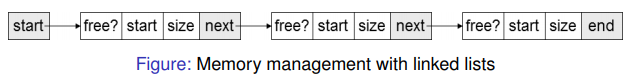
\includegraphics[scale=0.7]{linked_list.png}
\end{center}
\end{flushleft}

\pagebreak
\section*{Reference section} \label{sec:reference}
\begin{description}
	\item[placeholder] \hfill \\
\end{description}
\end{document}
